\documentclass{beamer}
\usetheme{CambridgeUS}

\usepackage{tikz}
\usepackage{xeCJK}
\usepackage{amsmath}
\usepackage[version=4]{mhchem}
\usetikzlibrary{graphs}
\usepackage{chemarr}
\usetikzlibrary{automata, arrows, positioning, calc}
\usepackage{fontspec}
\usepackage{caption}
\usepackage{subfigure}
\usepackage{graphicx}

% 英文字体配置部分
\setmainfont{Source Serif Pro}%Times New Roman
\setsansfont{Source Sans Pro}
\setmonofont{Source Code Pro}
% 中文字体配置部分
\usepackage{xeCJK}%中文字体
\setCJKmainfont{宋体}%正文字体
\setCJKsansfont{黑体}%无衬线字体
\setCJKmonofont{楷体}%等宽字体
\setCJKfamilyfont{boldsong}{Source Han Serif SC Heavy}

\title[单环马氏链环流的大偏差与涨落定理]{单环马氏链环流的大偏差与涨落定理} 
\author{姜瑜浩}

\institute[CSRC]
{\normalsize 指导老师:贾晨 教授\\
% \medskip
北京计算科学研究中心
% \textit{yuhaojiang@csrc.ac.cn}
} 
\begin{document}
	\frame{\titlepage}
	\begin{frame} {酶:生物系统中化学反应的催化剂}
		三步 Michaelis-Menten 酶动力学模型:
		$$
		E + S \xrightleftharpoons[k_{-1}]{k_1}
		ES \xrightleftharpoons[k_{-2}]{k_2}
		EP \xrightleftharpoons[k_{-3}]{k_3}
		E + P
		$$
		\begin{figure}[h]
			\centering
			\includegraphics[scale=0.4]{chart/enzyme.png}
	    \end{figure}
	\end{frame}

	\begin{frame}{酶:生物系统中化学反应的催化剂}
		相应的马氏链模型
		\begin{figure}[h]
			\centering
			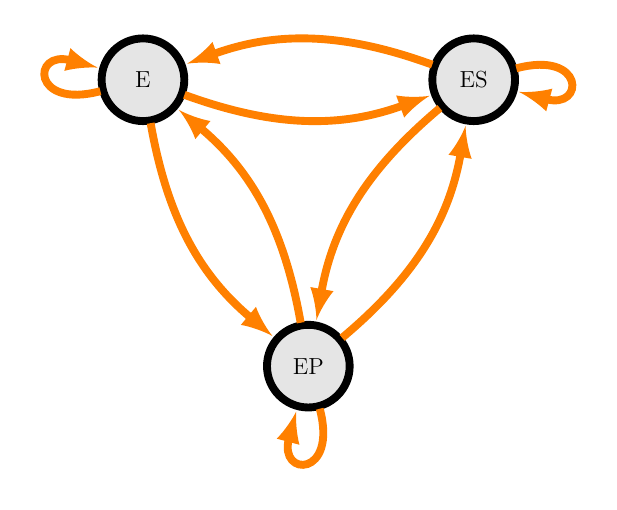
\begin{tikzpicture}[scale=0.7, font=\sffamily]
				\tikzstyle{every node} = [font=\large,scale=0.7]
				% Setup the style for the states
				\tikzset{node style/.style={state, 
											minimum width=1.5cm,
											line width=1mm,
											fill=gray!20!white}}
				% Draw the states
				\node[node style] at (0, 0)     (e)     {E};
				\node[node style] at (6, 0)     (es)     {ES};
				\node[node style] at (3, -5.196) (ep) {EP};
		
				% Connect the states with arrows
				\draw[every loop,
					  auto=right,
					  line width=1mm,
					  >=latex,
					  draw=orange,
					  fill=orange]
					(e)     edge[bend right=20]             (ep)
					(e)     edge[bend right=20, auto=left]  (es)
					(es)     edge[bend right=20]             (e)
					(es)     edge[bend right=20, auto=left]  (ep)
					(ep) edge[bend right=20]             (es)
					(ep) edge[bend right=20, auto=left]  (e)
					(e) edge[loop left] (e)
					(es) edge[loop right] (es)
					(ep) edge[loop below] (ep);
			\end{tikzpicture}
		\end{figure}
	\end{frame}

	\begin{frame}{马氏链中的环流}
		\begin{block}{为什么研究上述马氏链中的环?}
			考虑上述马氏链中,若环 $E \rightarrow EP \rightarrow ES \rightarrow E$ 出现的频率大于环 $E \rightarrow ES \rightarrow EP \rightarrow E$ 出现的频率,则化学反应整体向正反应进行,否则向负反应进行。
			通过研究马氏链中每个环出现的频率,可以研究化学反应整体方向以及反应进程。
		\end{block}
	\end{frame}

	\begin{frame}{马氏链中的环流}
		\begin{block}{环擦除定义下的环}
			\begin{table}[htb!]
				\renewcommand \arraystretch{1} \centering
				\scalebox{0.7}{
				\begin{tabular}{cccccccccc} \hline\hline
			   $n$            & 0 & 1 & 2 & 3   & 4     & 5 & 6 & 7         & 8 \\ \hline
			   $\xi_n$         & 1 & 2 & 3 & 3   & 2     & 3 & 4 & 1         & 4 \\ \hline
			   $\tilde{\xi}_n$& {[}1{]} & {[}1,2{]} & {[}1,2,3{]} & {[}1,2,3{]} & {[}1,2{]} & {[}1,2,3{]} & {[}1,2,3,4{]} & {[}1{]} & {[}1,4{]} \\ \hline
				\text{形成的环} &   &   &   & (3) & (2,3) &   &   & (1,2,3,4) &   \\ \hline\hline
				\end{tabular}}
				\caption{导出链的变化过程和轨道中形成的环}\label{trajectory}
			\end{table}
		\end{block}

	\end{frame}

	\begin{frame}{马氏链中的环流}
		\begin{block}{生成树定义下的环}

			
		\end{block}
		
	\end{frame}

	\begin{frame}{马氏链中的环流}
		\begin{block}{两种类型环的比较}

			
		\end{block}
		
	\end{frame}

	\begin{frame}{环流的大偏差原理}
		
	\end{frame}


















	\begin{frame}{马氏链的环流理论}
		\begin{block}{环流分布}
			设$(\mathit{X}_i)_{i\in \mathbb{N}}$是平稳不可约正常返马氏链,且转移概率矩阵为$\mathit{P}$,状态空间为有限集 $\Gamma$。对于该马氏链在$n>0$之前的序列,
			用 $\mathcal{C}_n$ 表示其中出现的环的集合,$\mathit{w}_{c,n}$ 表示其中环 $c$ 出现的次数。
			则当 $n \rightarrow +\infty$,随机变量序列 $(\mathcal{C}_n, \mathit{w}_{c, n})$会有:
			\begin{align*}
				\mathcal{C}_{\infty} &= \lim_{n \rightarrow +\infty} \mathcal{C}_n, \quad a.e. \\
				\mathit{w}_c &= \lim_{n \rightarrow +\infty} \frac{\mathit{w}_{c,n}}{n}, \quad a.e. 
			\end{align*}
			且环流分布为:
			$$
			\mathit{w}_c = \mathit{p}_{i_1, i_2} \mathit{p}_{i_2, i_3} \cdots \mathit{p}_{i_{s-1}, i_{s}} \mathit{p}_{i_s, i_1} \frac{\mathit{D}(\{i_1, i_2, \cdots i_s\}^c)}{\sum_{j\in \mathit{S}} \mathit{D}(\{j\}^c)}
			$$
			其中 $\mathit{D}(H)$ 是以集合 $H$ 为行和列的指标,$I-P$ 的主子式,且令 $\mathit{D}(\phi) = 1$。
		\end{block}
	\end{frame}

	\begin{frame}{大偏差理论}
		\begin{block}{大数定律}
			设独立同分布的随机变量序列 $\left(\mathit{X}_i \right)_{i\in \mathbb{N}}$ 定义于状态空间 $\Gamma=\{1, \cdots, r\}$,概率分布为 $\rho=(\rho_s)_{s \in \Gamma}$。定义 $\rho$ 所处的空间为:
			$$ 
			\mathfrak{M}_1(\Gamma) = \{\nu = (\nu_1, \nu_2, \cdots, \nu_r)\in [0,1]^r:\sum_{s=1}^r \nu_s = 1\}
			$$ 
			令经验测度$\mathit{L}_n = \frac{1}{n}\sum_{i=1}^{n}\delta_{\mathit{X}_i} $, 即 $\mathit{L}_n \in \mathfrak{M}_1(\Gamma)$,
			则根据大数定律,有
			\begin{figure}
				\centering
				\ce{$d(\mathit{L}_n, \rho)$ ->[$n\rightarrow \infty$] 0 $\quad$
				 $\mathbb{P} - a.s.$} 
			\end{figure}
			其中上述度量为全变差距离
			$$
			d(\mu, \nu) = \frac{1}{2} \sum_{s=1}^r |\mu_s - \nu_s|, \quad \mu, \nu \in \mathfrak{M}_1(\Gamma)
			$$
		\end{block}
	\end{frame}

	\begin{frame}{大偏差理论}
		\begin{block}{Level-1 大偏差 (Cramers 定理)}
			$(\mathit{X}_i)_{i\in \mathbb{N}}$是上述定义的独立同分布的随机变量序列,相应的经验测度为 $\mathit{L}_n = \frac{1}{n} \sum_{i=1}^n \delta_{\mathit{X}_i}$。那么,对于 $\forall a>0$,有:
			$$
			\lim_{n \rightarrow \infty} \frac{1}{n} \log \mathbb{P} \left(\mathit{L}_n \in \mathit{B}_a^c(\rho)\right) = -\inf_{\nu \in \mathit{B}_a^c(\rho)} \mathit{I}(x)
			$$
			其中 $\mathit{B}_a(\rho)=\{\nu \in \mathfrak{M}_1(\Gamma): d(\nu,  \rho) \le a\}$ 是 $\rho$ 的邻域,$\mathit{B}_a^c(\rho) = \mathfrak{M}_1(\Gamma) \backslash  \mathit{B}_a(\rho)$,且称
			$$
			\mathit{I}_{\rho}(\nu) = \sum_{s=1}^r \nu_s \log \left(\frac{\nu_s}{\rho_s}\right)
			$$
			为速率函数。
		\end{block}
	\end{frame}

	\begin{frame}{大偏差理论}
		\begin{block}{Level-2 大偏差 (Sanov定理)}
			在随机变量序列 $(\mathit{X}_i)_{i\in \mathbb{N}}$ 上,定义对经验测度
			$\mathit{L}_n^2 = \frac{1}{n} \sum_{i=1}^n \delta_{(\mathit{X}_i, \mathit{X}_{i+1})}$
			
			不妨令 $\mathit{X}_{n+1} = \mathit{X}_1$(当$n\rightarrow \infty$时,该假设对$\mathit{L}_n^2$ 取值无影响。)
			则 $\mathit{L}_n^2$ 所在的概率测度空间
			$\widetilde{\mathfrak{M}}_1(\Gamma \times \Gamma) = \{\nu=(\nu_{st}) \in \mathfrak{M}_1(\Gamma \times \Gamma):$ \\$ \sum_{t} \nu_{st} = \sum_{t} \nu_{ts}, \forall s\}.$
		
			Sanov 证明了对于 $\forall a > 0$,有:
			$$
			\lim_{n \rightarrow \infty} \frac{1}{n} \log \mathbb{P}(\mathit{L}_n^2 \in B_a^c(\rho \times \rho))
			= - \inf_{\nu \in B_a^c(\rho \times \rho)} \mathit{I}_{\rho}^2(\nu)
			$$
			其中 $B_a(\rho \times \rho) = \{\nu \in \widetilde{\mathfrak{M}}_1(\Gamma \times \Gamma): d(\nu, \rho \times \rho) \le a\}$,$\bar{\nu}_s = \sum_t \nu_{st}$,且速率函数为
			$$
			\mathit{I}_{\rho}^2(\nu) = \sum_{s,t} \nu_{st} \log\left(\frac{\nu_{st}}{\bar{\nu_s}\rho_t}\right)
			$$
		\end{block} 
	\end{frame}

	\begin{frame}{环流的大偏差理论}
		\begin{block}{环流的大偏差理论}
			考虑上述环流问题的随机过程 $(\mathit{X}_i)_{i\in \mathbb{N}}$,则 $C_{\infty}=\{c_1, c_2, \dots, c_s\}$ 为该过程所有可能环的集合,$\mathit{w} = \left(\mathit{w}_{c_1}, \mathit{w}_{c_2}, \dots, \mathit{w}_{c_s}\right)$ 为该马氏链的环流分布。不妨令 $\mathit{X}_{n+1} = \mathit{X}_1$,环流的经验测度为 $\mathit{w}_n = \left(\mathit{w}_{c_1, n}, \mathit{w}_{c_2, n}, \dots, \mathit{w}_{c_s, n}\right)$
			定义 $\mathit{w}_{c, n}$所在的空间:
			$$
			\mathfrak{M}_2 = \{\mu=\left(\mu_{c_1}, \mu_{c_2}, \dots, \mu_{c_s}\right)\in \left[0, 1\right]^s: \sum_{i=1} |c_i| \mu_{c_i}=1\}, 
			$$
			其中 $|c_i|$ 表示环 $c_i$ 中点的数量。
			则对 $\forall a >0$,有:
			$$
			\frac{1}{n} \log \mathbb{P} \left(\mathit{w}_n \in B_a^c(\mathit{w})\right) = - \inf_{\nu \in B_a^c(\mathit{w})} \mathit{I}^{c_1, c_2, \dots, c_s}(\nu)
			$$
		\end{block}
	\end{frame}

	\begin{frame}{速率函数}
		\begin{block}{Level-1 大偏差的速率函数}
			\begin{itemize}
				\item $\mathit{I}_{\rho}$ 是有界的,连续的,且在空间 $\mathfrak{M}_1(\Gamma)$是强凸的
				\item $\mathit{I}_{\rho} \ge 0$。当且仅当 $\nu = \rho$ 时,取等。
				\item 通常称 $\mathit{H}(\nu | \rho) = \mathit{I}_{\rho}$ 为 $\nu$ 关于 $\rho$ 的交叉熵。在信息论中,通常用其表示两个函数分布之间的差别。
			\end{itemize}
		\end{block}

		\begin{block}{Level-2 大偏差的速率函数}
			\begin{itemize}
				\item $\mathit{I}^2_{\rho}$ 是有界的,连续的,且在空间 $\widetilde{\mathfrak{M}}_1(\Gamma \times \Gamma)$ 是强凸的。
				\item $\mathit{I}^2_{\rho}(\nu) \ge 0$。当且仅当 $\nu = \rho \times \rho$ 时,取等。
				\item $\mathit{I}_{\rho}^2(\nu) = \mathit{H}(\nu | \bar{\nu} \times \rho)$为 $\nu$ 相对于 $\bar{\nu} \times \rho$ 的交叉熵。
			\end{itemize}
		\end{block}
	\end{frame}

	% \begin{frame}{主要难点}
	% 	给定一个图$G^n(k)$,考虑图中遍历所有边的欧拉回路,并计算出每种环出现的数量 $k=(k_c)_{c \in \mathcal{C}_{\infty}}$的欧拉回路数量 $\mathcal{E} (G^n(k))$。
	% 	\begin{figure}[h]
	% 		\centering
	% 		\includegraphics[scale=0.2]{graph1.png}
	% 		\caption*{马氏链诱导出的图}
	% 	\end{figure}
	% \end{frame}

	% \begin{frame}{难点简化}
	% 	针对酶动力学模型,下图所示的马氏链
	% 	\begin{figure}[h] \label{fi}
	% 		\centering
	% 		\includegraphics[scale=0.3]{n-state2.png}
	% 		\caption*{m状态马氏链诱导出的图}
	% 	\end{figure}
	% 	可以得出符合要求的欧拉回路数量:
	% 	\tiny{
	% 	\begin{align*}
	% 		\mathcal{E}_1 (G^m(k)) &= 
	% 		\binom{k_{12}+k_{1m}+k^{+}+k^{-}}{k_{12}, k_{1m}, k^{+}, k^{-}} 
	% 		\binom{k_{1}+k_{12}+k_{1m}+k^{+}+k^{-}}{k_{12}+k_{1m}+k^{+}+k^{-}}
	% 		\biggl[\Pi_{i\in S, i\neq 1} \binom{\sum_{c \ni i} k_{c} - 1}{\sum_{c \ni i} k_{c} - k_{i} - 1}\biggr]\\
	% 		&\biggl[\sum_{k_{23}^{+}+k_{23}^{-}=k_{23}} \sum_{k_{34}^{+}+k_{34}^{-}=k_{34}}
	% 		\dots \sum_{k_{m-1,m}^{+}+k_{m-1,m}^{-}=k_{m-1,m}}
	% 		\binom{k_{23}^{+}+k_{12}+k^{+}-1}{k_{23}^{+}} \binom{k_{34}^{+}+k_{23}^{+}+k^{+}-1}{k_{34}^{+}} \\
	% 		&\dots \binom{k_{m-1, m}^{+}+ k^{+}_{m-2, m-1} + k^{+}  -1}{k_{m-1, m}^{+}} \binom{k_{1, m} + k_{m-1, m}^{-} + k^{-} -1}{k_{m-1, m}^{-}} \binom{k_{m-1, m}^{-} + k_{m-2, m-1}^{-} + k^{-} - 1}{k_{m-2, m-1}^{-}} \\
	% 		&\dots \binom{k_{23}^{-} + k_{34}^{-} + k^{-} - 1}{k_{23}^{-}}\biggr]
	% 	\end{align*}}
	% \end{frame}

	\begin{frame}{速率函数}
		对于三状态马氏链,环流大偏差速率函数:
		\begin{align*}
			I_3^c(\nu) &= \sum_{c \in \mathcal{C}_{\infty}} \nu_{c} \log \frac{\nu_{c}}{w_c} + \sum_{i\in S}(\nu^i - \nu_i)\log \frac{\nu^i - \nu_i}{w^i - w_i} \\
			&-(\tilde{\nu} - \sum_{i\in S}\nu_i)\log(\frac{\tilde{\nu} - \sum_{i\in S}\nu_i}{\tilde{w} - \sum_{i\in I}w_i}) \\
			&-\sum_{i\in S} \nu^i \log (\frac{\nu^i}{w^i})
		\end{align*}

		\begin{figure}[h]
			\centering
			\includegraphics[scale=0.3]{3-state.png}
			\caption*{状态转移图}
		\end{figure}
	\end{frame}

	\begin{frame}{速率函数}
		对于三状态马氏链,净环流大偏差速率函数:
		\begin{align*}
			\bar{I}(\bar{\nu}) = \min_{\nu \in \bar{E}(\bar{\nu})} I^c_3(\nu)
		\end{align*}
		其中 $\bar{E}(\bar{\nu}) = \{\nu = (\nu_c)_{c \in \mathcal{C}_{\infty}} \in E | \nu_1 +\nu_2 +\nu_3 +2(\nu_{12} +\nu_{13} +\nu_{23}) +3(2\nu_{132} +\bar{\nu})=1\}$

		\begin{figure}[h]
			\centering
			\includegraphics[scale=0.3]{3-state.png}
			\caption*{状态转移图}
		\end{figure}
	\end{frame}

	\begin{frame}{速率函数}
		对于n状态马氏链,且状态间的转移概率非零的仅有$\{p_{i, i+1}, i=1, \dots n-1\} \bigcup \{p_{i, i-1}, i=2, \dots n-1\} \bigcup \{p_{n,1}\}$, 则相应的大偏差速率函数:
		\begin{align*}
			I_{m'}^{c}(\nu) = \sum_{i \in S} \sum_{c \ni i} \nu_c \log \left(\frac{\nu_c}{\nu^i} /\frac{w_c}{w^i}\right)
		\end{align*}
		\begin{figure}[h]
			\centering
			\includegraphics[scale=0.3]{n-state.png}
			\caption*{状态转移图}
		\end{figure}
	\end{frame}

	\begin{frame}{速率函数}
		\begin{block}{环流大偏差的速率函数}
			\begin{itemize}
				\item $\mathit{I}^{c_1, c_2, \dots, c_s}$ 是有界的,连续的,且是凸函数的。
				\item $\mathit{I}^{c_1, c_2, \dots, c_s}(\nu) \ge 0$。当且仅当 $\nu = w$ 时,取等。
				\item 如果 $c_k$ 和 $c_l$ 相似(环包含的节点相同),则有下式成立(涨落定理)
				\begin{align*}
					&\mathit{I}^{c_1, c_2, \dots, c_s}(x_1, \dots, x_k, \dots, x_l, \dots, x_r) \\
					&= \mathit{I}^{c_1, c_2, \dots, c_s}(x_1, \dots, x_l, \dots, x_k, \dots, x_r) - (\log \frac{\gamma^{c_k}}{\gamma^{c_l}} (x_k - x_l))
				\end{align*}
				其中对于$c = (i_1, i_2, \dots, i_s)$, 定义$\gamma^c = p_{i_1 i_2} p_{i_2 i_3} \dots p_{i_s i_1}$。
			\end{itemize}
		\end{block}
	\end{frame}
	% \begin{frame}{速率函数}
	% 	\begin{block}{净环流大偏差的速率函数}
	% 		令 $c_l$ 表示环 $E \longrightarrow EP \longrightarrow ES \longrightarrow E$,$c_l^-$ 表示相应的反环 $E \longrightarrow ES \longrightarrow EP \longrightarrow E$,称$\mathit{w}_{c_l} - \mathit{w}_{c_l^-}$为净环流。
	% 		对于上述酶促反应,净环流趋于平稳,已经是达到动态平衡。依据大偏差的收缩原则,可以证明净环流大偏差是存在的,但净环流的具体表达式依旧值得研究?
	% 	\end{block}

	% 	\begin{block}{该研究的主要意义}
	% 		通过分析不可逆马氏链中环的性质,可以更好地理解各种随机生化系统的不可逆性。
	% 		以统计力学的角度,涨落定理可以准确的量化生化系统稀有事件发生的概率。
	% 		对于上述酶促反应,关于环流的涨落定理可以通过求解大偏差中的速率函数清晰得到。
	% 		所以该研究对于理解随机生化系统有着重要意义
	% 	\end{block}
	% \end{frame}

	% \begin{frame}{酶促反应}
	% 	没有化学反应酶参与的动力学模型
	% 	$$
	% 	S \xrightleftharpoons[k_{-1}]{k_1} P
	% 	$$
	% 	两步 Michaelis–Menten 动力学模型
	% 	$$
	% 	E + S \xrightleftharpoons[k_{-1}]{k_1}
	% 	ES \xrightleftharpoons[k_{-2}]{k_2}
	% 	EP 
	% 	$$
	% 	三步 Hill 动力学模型
	% 	$$
	% 	E + S \xrightleftharpoons[k_{-1}]{k_1}
	% 	ES \xrightleftharpoons[k_{-2}]{k_2}
	% 	EP \xrightleftharpoons[k_{-3}]{k_3}
	% 	E + P
	% 	$$
	% 	推广到 $n$ 步的动力学模型
	% 	$$
	% 	E + S \xrightleftharpoons[k_{-1}]{k_1}
	% 	ES \xrightleftharpoons[k_{-2}]{k_2}
	% 	EP_1 \xrightleftharpoons[k_{-3}]{k_3}
	% 	EP_2 \xrightleftharpoons[k_{-4}]{k_4}
	% 	\cdots
	% 	EP_{n-2} \xrightleftharpoons[k_{-n}]{k_n}
	% 	E + P
	% 	$$
	% \end{frame}

	% \begin{frame}{其他生化反应}
	% 	如果已知上述环流大偏差的表达式,能否推广到其他生化反应?
	% 	\captionsetup[figure]{labelfont={bf},name={},labelsep=period}
	% 	\begin{figure}[h]
	% 		\begin{minipage}[t]{0.4\linewidth}
	% 			\centering
	% 			\includegraphics[scale=0.4]{phosphorylation_dephosphorylation_cycle.png}
	% 			\caption{磷酸-脱磷酸化循环}
	% 		\end{minipage}
	% 		\begin{minipage}[t]{0.4\linewidth}
	% 			\centering
	% 			\includegraphics[scale=0.4]{general_modifier_machanism.png}
	% 			\caption{广义的修正机制}
	% 		\end{minipage}
	% 		%\caption{四状态生化反应模型}
	%     \end{figure}
		
	% 	\begin{figure}[h]
	% 		\begin{minipage}[t]{0.4\linewidth}
	% 			\centering
	% 			\includegraphics[scale=0.4]{De Young-Keizer model.png}
	% 			\caption{De Young-Keizer 模型}
	% 		\end{minipage}
	% 		\begin{minipage}[t]{0.4\linewidth}
	% 			\centering
	% 			\includegraphics[scale=0.4]{MWC.png}
	% 			\caption{MW模型}
	% 		\end{minipage}
	% 		%\caption{八状态生化反应模型}
	%     \end{figure}
	% \end{frame}

	% \begin{frame}{总结}
	% 	主要解决的问题
	% 	\begin{itemize}
	% 		\item 三状态马氏链环流大偏差中的速率函数表达式的求解
	% 		\item 把三状态的结果推广到 $n$ 状态的酶促反应
	% 		\item 上述马氏链的净环流大偏差中的速率函数表达式的求解
	% 		\item 验证上述表达式中的速率函数是否符合涨落定理
	% 	\end{itemize}
	% \end{frame}
	
	\begin{frame}
		\begin{center}
			\Huge 谢谢!
		\end{center}
	\end{frame}
\end{document}